%----------------------------------------
\section{Linear Real and Integer Arithmetic}
%----------------------------------------

Our solver for linear arithmetic is based on a variant of the Simplex
approach~\cite{Dutertre2006}.  A theory conflict is a conjunction of
literals $\ell_j$ of the form $\sum_i a_{ij} x_{i} \leq b_j$.  The
proof of unsatisfiability is given by Farkas coefficients $k_j\geq 0$
for each inequality $\ell_j$.  These coefficients have the properties
$\sum_j k_ja_{ij} = 0$ and $\sum_j k_jb_j < 0$.  In the following we
use the notation of adding inequalities (provided the coefficients are
positive).  Thus, we write $\sum_j k_j \ell_j$ for $\sum_i (\sum_j k_j
a_{ij}) x_i \leq \sum_j k_jb_j$. With the property of the Farkas
coefficients we get a contradiction ($0<0$) and this shows that the theory
conflict is unsatisfiable.

A conjunction of literals may have rational but no integer solutions.
In this case, there are no Farkas coefficients that can prove the
unsatisfiability.  So for the integer case, our solver may introduce
extended branches~\cite{Dillig2011}, which are just branches of the DPLL engine
on newly introduced literals.  In the proof tree this results in resolution
steps with these literals as pivots.

%% -*- latex-mode -*-
\begin{example}
  The formula $t \leq 2a \leq r \leq 2b+1 \leq t$ has no integer
  solution but a rational solution.  Introducing the branch $a\leq b
  \lor b < a$ leads to the theory conflicts $t\leq 2a \leq 2b \leq
  t-1$ and $r \leq 2b+1 \leq 2a-1 \leq r-1$ (note that $b<a$ is
  equivalent to $b+1 \leq a$).  The corresponding proof tree is given
  below.  The Farkas coefficients in the theory lemmas are given in
  parenthesis.  Note that the proof tree shows the clauses, i.\,e.,
  the negated conflicts.  A node with more than two parents denotes that
  multiple applications of the resolution rule are taken one after another.

  \centerline{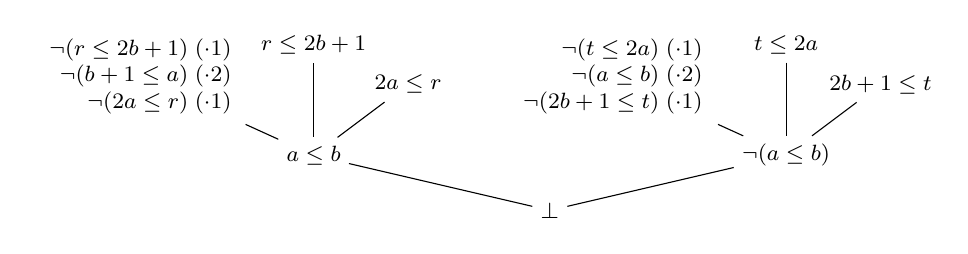
\begin{tikzpicture}\footnotesize
    \node (t2) at(0,0) {$\begin{array}{r}\lnot(r\le 2b+1)\;(\cdot 1)\\\lnot
        (b+1\le a)\;(\cdot 2)\\\lnot(2a\le r)\;(\cdot 1)\end{array}$};
    \node (t1) at(6,0) {$\begin{array}{r}
                          \lnot(t\le 2a)\;(\cdot 1)\\
                          \lnot(a\le b)\;(\cdot 2)\\
			  \lnot(2b+1\le t)\;(\cdot 1)
			  \end{array}$};
    \node (i21) at(2.2,.4) {$r\leq 2b+1$};
    \node (i22) at(3.4,-.1) {$2a\leq r$};
    \node (i11) at(8.2,.4) {$t\leq 2a$};
    \node (i12) at(9.4,-.1) {$2b+1\leq t$};
    \node (r2) at(2.2,-1) {$a\le b$};
    \node (r1) at(8.2,-1) {$\lnot(a\le b)$};
    \node (b) at(5.2,-1.7) {$\bot$};
    \draw (t1)-- (r1);
    \draw (i11)-- (r1);
    \draw (i12)-- (r1);
    \draw (t2)-- (r2);
    \draw (i21)-- (r2);
    \draw (i22)-- (r2);
    \draw (r1)-- (b);
    \draw (r2)-- (b);
  \end{tikzpicture}}

Now consider the problem of deriving an interpolant between $A\equiv t\le
2a\le r$ and $B\equiv r\le 2b+1\le t$.  We can obtain an interpolant by
annotating the above resolution tree with partial interpolants.  
To compute a partial interpolant for the theory lemma
$\lnot(r\le 2b+1) \lor \lnot(b+1\le a) \lor \lnot(2a\le r)$,
we purify the \emph{negated} clause according to the definition in
Section~\ref{sec:purification}, which gives
\[ r\le 2b+1  \land  x_1 \le a \land -x_1 + b + 1 \le 0 \land 2a\le r. \]
Then, we sum up the $A$-part of the conflict (the second
and fourth literal) multiplied by their corresponding Farkas coefficients.
This yields the interpolant $2x_1 \le r$.
Similarly, the negation of the theory lemma 
$\lnot(t\le 2a) \lor \lnot(a\le b) \lor  \lnot(2b+1\le t)$ is purified to
\[t\le 2a \land x_2+a\le 0 \land -x_2\le b \land  2b+1\le t,\]
which yields the partial interpolant $2x_2+t \le 0$.  
Note, that we have to introduce different variables for each literal.
Intuitively, the variable $x_1$ stands for $a$ and $x_2$ for $-a$.  
Using Pudl\'ak's algorithm we can derive the same interpolants for 
the clause $a\leq b$ resp.\ $\lnot (a\leq b)$.

For the final resolution step, the two partial interpolants 
$2x_1 \le r$ and $2x_2+t \le 0$ are combined into
the final interpolant of the problem.
Summing up these inequalities with $x_1=-x_2$ we get $t\le r$.  
While this follows from $A$, it is not
inconsistent with $B$.  We need an additional argument that, given $r=t$,
$r$ has to be an even integer.  This also follows from the partial
interpolants when setting $x_1=-x_2$: $t\leq -2x_2 = 2x_1 \leq r$.
\ifnewinterpolation
The final interpolant computed by our algorithm is 
$t \leq 2\floorfrac{r}{2}$.
\else
The final interpolant computed by our algorithm is 
$t \leq r \land (t \geq r \rightarrow t \leq 2\lfloor r/2\rfloor)$.
\fi

%Using the Strong-Weak-Interpolation lemma we have to find I3 such that
%(ALL x_1 x_2.   x_1 \le a --> 2x_1 \le r  
%           &&  x_2 +a \le 0 --> 2x_2 + t \le 0) --> I3
%and
%I3 --> (EX x_1 x_2. -x_1 + b + 1 \le 0 && 2x_1 \le r  
%                  ||  -x_2  \le b && 2x_2 + t \le 0)


In general, we can derive additional constraints on the variables
if the constraint resulting from summing up the two partial interpolants
holds very tightly. We know implicitly that $x_1=-x_2$ is an integer
value between $t/2$ and $r/2$.  If $t$ equals
$r$ or almost equals $r$ there are only a few possible values which we can
explicitly express using the division function as in the example above.
\ifnewinterpolation
We assume that the (partial) interpolant $F$ always has a certain
property.  There is some term $s$ and some constant $k$, such that
for $s > 0$ the interpolant is always false and for $s < -k$ the
interpolant is always true (in our case $s = t-r$ and $k = 0$). 
For a partial interpolant that still contains auxiliary variables $\vec x$,
we additionally require that $s$ contains them with a positive coefficient
and that $F$ is monotone on $\vec x$, i.\,e., $\vec x \geq \vec x'$ implies
$F(\vec x) \rightarrow F(\vec x')$.
\else
This leads to the general form $t-r\leq 0\land (t-r\geq
-k\rightarrow F)$.  In our example we have $k=0$ and $F$ specifies
that $r=t$ is even.
\fi
\end{example}

%%  LocalWords:  interpolant interpolants




%TODO as in \cite{Dillig2011}.
%FIXME end

%\begin{tikzpicture}[thick]
%    \draw(0,0)--(12.5,0);
%    \foreach \x/\xtext in {0/0,3/1,6/2,9/3,12/4}
%      \draw(\x,0pt)--(\x,3pt) node[above] {\xtext};
%    \foreach \x in {0,1,...,12}
%      \draw(\x,0pt)--(\x,-3pt) node[below] {$\frac{\x}{3}$};
%\end{tikzpicture}

% (minimal) template-picture for illustrating the eq-stuff
%\begin{tikzpicture}
% \draw(0,0)--(10,0);
% \node [above] (s2) at (2,0) {$\frac{s_2}{c_2}$};
% \node [above] (s1) at (8,0) {$-\frac{s_1}{c_1}$};
% \draw let \p1 = (s2) in (\x1,-3pt)--(\x1,3pt);
% \draw (8,-3pt)--(8,3pt);
% \draw [decoration={brace,mirror},
%    decorate] 
%    (6,0) -- (8,0) node[pos=0.5,below] {$\frac{k_1}{c_1}$}; 
%\end{tikzpicture}

%in integer context, $\varepsilon$ means 1, usually... %TODO genau festlegen


To mechanise the reasoning used in the example above, our resolution
rule for mixed inequality literals requires that the interpolant patterns
that label the clauses have a certain shape.  An auxiliary
variable of a mixed inequality literal may only occur in the 
interpolant pattern
if the negated literal appears in the clause.  Let $\vec x$ denote the
set of auxiliary variables that occur in the pattern.  We require 
that these
variables only occur inside a special sub-formula of the form $LA(s(\vec x), k,
F(\vec x))$.  The first parameter $s$ is a linear term over the
variables in $\vec x$ and arbitrary other terms not involving $\vec
x$.  The coefficients of the variables $\vec x$ in $s$ must all be
positive.  The second parameter $k\in \mathbb{Q}_\eps$ is a
constant value.  In the real case we only allow the values $0$ and
$-\eps$. In the integer case we allow $k\in\mathbb{Z}, k\geq -1$.  
To simplify the presentation, we sometimes write $-\eps$ for $-1$ in the integer case.
The third parameter $F(\vec x)$ is a formula that contains the variables
from $\vec x$ at arbitrary positions.
\ifnewinterpolation
We require that $F$ is monotone, i.\,e., $\vec x \geq \vec x'$ implies 
$F(\vec x) \rightarrow F(\vec x')$.  
Moreover, $F(\vec x)=\bot$ for $s(\vec x) > 0$ and
$F(\vec x)=\top$ for $s(\vec x) < -k$.  The sub-formula
$LA(s(\vec x), k, F(\vec x))$ stands for $F(\vec x)$ and it is only
used to remember what the values of $s$ and $k$ are.

The intuition behind the formula $LA(s(\vec x), k, F(\vec x))$ is that
$s(\vec x) \leq 0$ summarises the inequality chain that follows from the $A$-part of
the formula.  On this chain there may be some constraints on
intermediate values.  In the example above the $A$-part contains the
chain $t \leq 2a \leq r$, which is summarised to $s \leq 0$ (with $s=t-r$).
Furthermore the $A$-part implies that there is an even integer value between
$t$ and $r$.  If $s < -k$ (with $k=0$ in this case),  $t$ and $r$ are 
distinct, and there always is an even integer between them.
However, if $-k \leq s \leq 0$, the truth value of the interpolant depends on 
whether $t$ is even. 
\else
Again we have a strong and a weak
partial interpolant that are obtained by using different definitions
for $LA$.  These definitions are
\begin{align*}
LA\S\left(s(\vec x), k, F(\vec x)\right) &:\equiv
  \forall \vec x' \leq \vec x.~ LA^*(s(\vec x'),k,F(\vec x')) \\
LA\W \left(s(\vec x),k,F(\vec x)\right) &:\equiv
  \exists \vec x' \geq \vec x.~ LA^*(s(\vec x'),k,F(\vec x')) \\
\text{where}\quad
LA^*(s(\vec x'),k,F(\vec x')) &:\equiv
s(\vec x') \leq 0 \land 
  (s(\vec x') \geq -k \rightarrow F(\vec x'))
\end{align*}

The intuition behind the formula $LA^*(s(\vec x), k, F(\vec x))$ is that
$s(\vec x) \leq 0$ summarises the inequality chain that follows from the $A$-part of
the formula.  On this chain there may be some constraints on
intermediate values.  In the example above the $A$-part contains the
chain $t \leq 2a \leq r$, which is summarised to $t\leq r$.
Furthermore the $A$-part implies that there is an even integer value between
$t$ and $r$.  If $t$ and $r$ are distinct, this is no problem.
However, if $t \geq r$ we need that $t$ is even. Using the above
pattern we can choose $k=0$ and $F$ as the formula that states that
$t$ is even.  

To see that the strong interpolant $LA\S(s,k,F)$ implies the weak
interpolant $LA\W(s,k,F)$, instantiate $\vec x'$ with $\vec x$ in both 
formulae.
Having quantifiers in
the interpolant is no problem; once all mixed literals are resolved,
all auxiliary variables
are removed.  Then, the strong and weak interpolant are identical and have
no quantifiers.

\begin{techreport}
\begin{lemma} \label{lemma_las_implies_law}
  For all $s(\vec x),F(\vec x)$, the strong interpolant implies the weak one:
\[  LA\S(s(\vec x),k,F(\vec x)) \rightarrow LA\W(s(\vec x),k,F(\vec x))\]
\end{lemma}
\begin{proof}
  Instantiate the vector $\vec x'$ in $LA\S$ and $LA\W$ with $\vec x$.\qed
\end{proof}
\end{techreport}
\fi

In the remainder of the section, we will give the interpolants for the
leaves produced by the linear arithmetic solver and for the resolvent of the
resolution step where the pivot is a mixed linear inequality.

\subsection{Leaf Interpolation}

As mentioned above, our solver produces for a clause $C\equiv\lnot
\ell_1\lor \dots \lor\lnot \ell_m$ some Farkas coefficients
$k_1,\dots,k_m\geq 0$ such that $\sum_j k_j \ell_j$ yields a
contradiction $0 < 0$.  A partial interpolant for a theory lemma can be
computed by summing up the $A$-part of the conflict: $I$ is defined as
$\sum_j k_j (\ell_j \proj A)$~(if $\ell_j\proj A = \top$ we regard it
as $0\leq 0$, i.\,e., it is not added to the sum).  It is a valid interpolant as it
clearly follows from $\lnot C\proj A \iff \ell_1\proj A \land \dots
\land \ell_m\proj A$.  Moreover, we have that $I + \sum_j
k_j(\ell_j\proj B)$ yields $0< 0$, since for every literal, even
for mixed literals, $\ell_j\proj A + \ell_j\proj B = \ell_j$
holds\footnote{Strictly speaking this does not hold for shared literals, where
  $\ell\proj A = \ell\proj B = \ell$.  In that case use $k_j=0$ in
$I+\sum_j k_j(\ell_j\proj B)$ to see that $I$ is indeed a partial interpolant.}.  This
shows that $I\land \lnot C\proj B$ is unsatisfiable.

The linear constraint $\sum_j k_j (\ell_j \proj A)$ can be expressed
as $s(\vec x) \leq 0$.  Thus, we can equivalently write this
interpolant in our pattern as $LA(s(\vec x), -\eps,
\ifnewinterpolation s(\vec x) \leq 0 \else \bot\fi)$.  Since the
%JC: Changed -1 to -\eps in above line
Farkas coefficients are all positive and the auxiliary variables
introduced to define $\ell \proj A$ for mixed literals contain $x$
positively, the resulting term $s(\vec x)$ will also always contain
$x$ with a positive coefficient.

\paragraph{Theory combination lemmas.}

As mentioned in the preliminaries, we use theory combination clauses
to propagate equalities from and to the Simplex core of the linear
arithmetic solver.  These clauses must also be labelled with partial interpolants.
\begin{techreport}
In the following we give interpolants for those theory combination lemmas.
We will start with the case where no mixed literals occur, and treat lemmas
containing mixed literals afterwards.
\end{techreport}
\begin{tacas}The interesting case is when these clauses contain mixed literals.%, see
Table~\ref{tbl:iplthcomb} shows the corresponding partial interpolants.
The non-mixed case is given in the technical report.
    
The interpolant for the clause $a=b\lor a< b \lor a> b$ deserves more
explanation.  This clause is used to propagate equalities from the
linear arithmetic solver if it can derive $a\leq b$ and $b\leq a$.  In the
interpolant, $x_1$ is the variable with $b \leq x_1 \leq a$, and $x_2$
the variable with $a \leq -x_2 \leq b$.  The formula
$LA(x_1+x_2,0,EQ(x,x_1))$ basically states that $x_1 \leq -x_2$ and
that if $x_1\geq -x_2$ then $x_1$ equals the shared value $x$ of the
equality $a=b$.  We stress that the interpolant has the required form:
$x_1$ and $x_2$ only occur inside an $LA$ and with the correct
coefficients in $x_1+x_2$ while $x$ only occurs as first parameter of an
$EQ$ term, which appears positively in the negation normal form (by
the definition of $LA\S$ and $LA\W$).

\begin{table}[t]
  \begin{minipage}{.5\textwidth}
  Clause $C$: $a \neq b \lor a\leq b$\\
  $\lnot C\proj A$: $\ifnewinterpolation a=x \else a=x_a\land x_a=x_b\fi
                     \land -a+x_1\leq 0$\\
  $\lnot C\proj B$: $\ifnewinterpolation x=b \else x_a=x_b\land x_b=b\fi
                     \land -x_1+b< 0$\\
  Interpolant $I$: $LA(-x+x_1, -\eps, 
                    \ifnewinterpolation x_1 \leq x\else \bot\fi)$
  \end{minipage}%
  \begin{minipage}{.5\textwidth}
  Clause $C$: $a \neq b \lor a\geq b$\\
  $\lnot C\proj A$: $\ifnewinterpolation a=x \else a=x_a\land x_a=x_b\fi
                     \land a+x_2 \leq 0$\\
  $\lnot C\proj B$: $\ifnewinterpolation x=b \else x_a=x_b\land x_b=b\fi
                     \land -x_2-b< 0$\\
  Interpolant $I$: $LA(x+x_2, -\eps, 
                    \ifnewinterpolation x \leq -x_2\else \bot\fi)$
  \end{minipage}\\[6pt]
  \centerline{\begin{minipage}{.8\textwidth}
  Clause $C$: $a = b \lor a < b \lor a > b$\\
  $\lnot C\proj A$: $\ifnewinterpolation p_x \xor a=x 
                     \else a=x_a\land x_a \neq x_b\fi
                     \land -a+x_1\leq 0 \land a+x_2\leq 0$\\
  $\lnot C\proj B$: $\ifnewinterpolation \lnot p_x \xor x=b 
                     \else x_a \neq x_b\land x_b = b\fi
                    \land -x_1+b\leq 0 \land -x_2 - b\leq 0$\\
  Interpolant $I$: $LA(x_1+ x_2, 0, EQ(x, x_1))$
  \end{minipage}}\\%Just a little bit more space

  \caption{Interpolation of mixed theory combination clauses. We
    assume $a$ is $A$-local, $b$ is $B$-local, $a-b\leq 0$ has the
    auxiliary variable $x_1$, $b-a\leq 0$ has the auxiliary variable
    $x_2$ and $a=b$ the auxiliary variables $x_a$ and $x_b$. \label{tbl:iplthcomb}}
\end{table}
\end{tacas}


\begin{techreport}
\paragraph*{Interpolation of Non-Mixed Theory Combination Lemmas.}

If a theory combination lemma $t=u \lor t< u \lor t> u$ or $t \neq u \lor
t\leq u$ contains no mixed literal, we can compute partial interpolants as
follows.  If all literals in the clause are $A$-local, the formula $\bot$ is a
partial interpolant.  If all literals are $B$-local, the formula $\top$ is a
partial interpolant.  These are the same interpolants Pudl\'ak's algorithm
would give for input clauses from $A$ resp.\ $B$.

Otherwise, one of the literals belongs to $A$ and one to $B$.  The
symbols $t$ and $u$ have to be shared between $A$ and $B$ since they
appear in all literals.  We can derive a partial interpolant by
conjoining the negated literals projected to the $A$ partition.
\begin{align*}
  I &\equiv (t\neq u)\proj A \land (t\geq u)\proj A \land (t \leq u) \proj A. 
  &&\quad \mbox{for }t=u \lor t< u \lor t> u\\
  I &\equiv (t = u)\proj A \land (t > u) \proj A
  &&\quad \mbox{for }t\neq u \lor t\leq u
\end{align*}

Since we defined $I$ as $\lnot C \proj A$, the first property of the partial
interpolant holds trivially.  Also $I \land \lnot C \proj B$ is equivalent to
$\lnot C$ and therefore false.  The symbol condition is satisfied as $t$ and
$u$ are shared symbols.
\bigskip

\paragraph*{Interpolation of AB-Mixed Theory Combination Lemmas.}

\begin{table}[t]
  \begin{varwidth}{.5\textwidth}
  Clause $C$: $a \neq b \lor a\leq b$\\
  $\lnot C\proj A$: $\ifnewinterpolation a=x \else a=x_a\land x_a=x_b\fi
                     \land -a+x_1\leq 0$\\
  $\lnot C\proj B$: $\ifnewinterpolation x=b \else x_a=x_b\land x_b=b\fi
                     \land -x_1+b< 0$\\
  Interpolant $I$: $LA(-x+x_1, -\eps, 
                    \ifnewinterpolation x_1 \leq x\else \bot\fi)$
  \end{varwidth}\hfill
  \begin{varwidth}{.5\textwidth}
  Clause $C$: $a \neq b \lor a\geq b$\\
  $\lnot C\proj A$: $\ifnewinterpolation a=x \else a=x_a\land x_a=x_b\fi
                     \land a+x_2 \leq 0$\\
  $\lnot C\proj B$: $\ifnewinterpolation x=b \else x_a=x_b\land x_b=b\fi
                     \land -x_2-b< 0$\\
  Interpolant $I$: $LA(x+x_2, -\eps, 
                    \ifnewinterpolation x \leq -x_2\else \bot\fi)$
  \end{varwidth}\\[6pt]
  \centerline{\begin{varwidth}{.8\textwidth}
  Clause $C$: $a = b \lor a < b \lor a > b$\\
  $\lnot C\proj A$: $\ifnewinterpolation (p_x \xor a=x)
                     \else a=x_a\land x_a \neq x_b\fi
                     \land -a+x_1\leq 0 \land a+x_2\leq 0$\\
  $\lnot C\proj B$: $\ifnewinterpolation (\lnot p_x \xor x=b)
                     \else x_a \neq x_b\land x_b = b\fi
                    \land -x_1+b\leq 0 \land -x_2 - b\leq 0$\\
  Interpolant $I$: $LA(x_1+ x_2, 0, 
  \ifnewinterpolation x_1\leq -x_2 \land (x_1\geq -x_2 \rightarrow EQ(x, x_1))
  \else EQ(x, x_1)\fi)$
  \end{varwidth}}\\%Just a little bit more space
%
  \caption{Interpolation of mixed theory combination clauses. We
    assume $a$ is $A$-local, $b$ is $B$-local, $a-b\leq 0$ has the
    auxiliary variable $x_1$, $b-a\leq 0$ has the auxiliary variable
    $x_2$ and $a=b$ the auxiliary variables 
    \ifnewinterpolation $x$ and $p_x$\else $x_a$ and $x_b$\fi.
    \label{tbl:iplthcomb}}
\end{table}

If we are in the mixed case, all three literals are mixed. One of the two
terms must be $A$-local (in the following we denote this term by $a$) the
other term $B$-local (which we denote by $b$). To purify the literals, we introduce a fresh auxiliary
variable for each literal. Table~\ref{tbl:iplthcomb} depicts all possible mixed
theory lemmas together with the projections $\lnot C \proj A$ and $\lnot C
\proj B$ and a partial interpolant of the clause.

\begin{lemma}
The interpolants shown in Table~\ref{tbl:iplthcomb} are correct
partial interpolants of their respective clauses.
\end{lemma}

\begin{proof}
  First, we convince ourselves that these interpolants are of the right form:  The
  variables $x_1$ and $x_2$ appear in the first parameter of $LA$ with positive
  coefficients.  For the first two clauses that contain the literal $a\neq b$,
  the interpolant is allowed to contain $x$ at arbitrary positions.  
  \ifnewinterpolation Note that in the first interpolant
  $x_1\leq x$ is false for $-x+x_1 > 0$ and true for $-x+x_1 <\eps$, 
  i.\,e., $-x+x_1 \leq 0$.  Also, $x_1 \geq x_1'$ implies 
  $x_1\leq x \rightarrow x_1' \leq x$.  Similarly, for the second interpolant.

  In the
  third clause,
  $F(x_1,x_2) = x_1\leq -x_2 \land (x_1\geq -x_2 \rightarrow EQ(x, x_1))$ 
  is false for $x_1 + x_2 > 0$ (because of the first conjunct) and true 
  for $x_1 + x_2 < 0$ (because the implication holds vacuously).
  Also, $x_1 \geq x_1'$ and $x_2 \geq x_2'$ implies 
  $F(x_1,x_2) \rightarrow F(x_1', x_2')$.  To see this, note that
  $F(x_1,x_2)$ is false if $x_1' \geq -x_2'$ and $x_1' \neq x_1$.
  The variable $x$ appears only in an $EQ$-term which occurs
  positively in the partial interpolant. 
  \else  
  In the
  third clause the variable $x$ appears only in an $EQ$-term which occurs
  positively in the expanded form of the partial interpolant. 
  \fi

  Next we show
  \begin{align*}
    &\lnot C \proj A \models I\S \tag{Inductivity}\\
    &\lnot C \proj B \land I\W \models \bot \tag{Contradiction}
  \end{align*}

  \subsubsection*{Inductivity.}  
  \ifnewinterpolation
  For the clause $a\neq b\lor a\leq b$, the interpolant follows 
  from $\lnot C\proj A$, as $a=x$ and $-a + x_1 \leq 0$
  imply $x_1\leq x$. Similarly for the clause $a\neq b\lor a\geq b$,
  $\lnot C\proj A$ contains
  $a=x$ and $a + x_2 \leq 0$, which implies $x \leq -x_2$.
  \else
  For the clauses $a\neq b\lor a\leq b$ and $a\neq b\lor a\geq b$ the argument
  is symmetric.  We show only the case $C \equiv a\neq b \lor a\leq b$. 
  Assume $\lnot C\proj A$ and show $LA\S(-x_a+x_1,-\eps,\bot)$:
  \[
  \forall x_1' \leq x_1.~ -x_a+x_1' \leq 0 \land 
  (-x_a+x_1' \geq \eps \rightarrow \bot)
  \]
  Let $x_1'\leq x_1$. From $\lnot C \proj A$ we have $-a+x_1\leq 0$ and
  $a=x_a$. Hence, $-x_a + x_1' \leq 0$ as desired, which also shows that the
  implication in the second conjunct holds vacuously.

  \fi
  Now consider the clause $a= b\lor a< b \lor b< a$.
  \ifnewinterpolation
  Here, $\lnot C\proj A$ implies $x_1\leq -x_2$ and 
  that if $x_1\geq -x_2$ holds, then $x_1 = a =-x_2$. 
  Hence, $x_1\leq -x_2 \land x_1 \geq -x_2 \rightarrow EQ(x, x_1)$ holds.
  \else
  We assume $\lnot C\proj A$ and show $LA\S(x_1+x_2,0,x_a=x_1)$:
  \[\forall x_1' \leq x_1, x_2' \leq x_2.~ 
  x_1'+x_2' \leq 0 \land (x_1'+x_2' \geq 0 \rightarrow x_a = x_1').\]
  Let $x_1'\leq x_1$ and $x_2'\leq x_2$. 
  From $\lnot C\proj A$ we have $x_1 \leq a$ and $a+x_2\leq 0$.
  Thus, $x_1'+x_2' \leq x_1+x_2 \leq a + (-a) = 0$.
  Moreover, if $x_1'+x_2' \geq 0$ then
  \[ a\leq -x_2 \leq -x_2' \leq x_1' \leq x_1 \leq a,\]
  hence $a=x_1$.  With $a=x_a$ (also a part of $\lnot C \proj A$),
  this yields $x_a=x_1$.
  This shows that $LA\S(x_1+x_2,0,x_a=x_1)$ holds.
  \fi
  
  \subsubsection*{Contradiction.}
  Again we only show the first and third case. For the clause
  $C \equiv a\neq b \lor a\leq b$,
  \ifnewinterpolation
  note that $\lnot C\proj B$ and $LA\W(-x+x_1,-\eps,x_1 \leq x)$ 
  give the contradiction $x_1 > b = x > x_1$.
  For the clause $C \equiv a= b\lor a< b \lor b< a$,
  $\lnot C\proj B$ implies $x_1 \geq b \geq -x_2$. 
  With $x_1\leq -x_2$ from the interpolant this gives $x_1 = b$. Also,
  $x_1\geq -x_2\rightarrow EQ(x, x_1)$ from the interpolant gives
  $p_x \xor x=b$.  This is in contradiction with 
  $\lnot p_x \xor x=b$ from $\lnot C\proj B$.
  
  \else
  assume $\lnot C\proj B$ and $LA\W(-x_b+x_1,-\eps,\bot)$ hold:
  \[
  \exists x_1' \geq x_1.~ -x_b+x_1' \leq 0 \land (-x_b+x_1' \geq \eps \rightarrow \bot)
  \]
  Choose $x_1'$ for which the above formula holds. 
  From $\lnot C\proj B$ we have $-x_1+b < 0$ and
  $x_b=b$. Hence, $-x_b + x_1' \geq -b + x_1 > 0$.  This contradicts $-x_b+x_1'
  \leq 0$.
 
  Now consider the clause $C \equiv a= b\lor a< b \lor b< a$.
  We assume $\lnot C\proj B$ and $LA\W(x_1+x_2,0,x_b\neq x_1)$
  \[\exists x_1' \geq x_1, x_2' \geq x_2.~ 
  x_1'+x_2' \leq 0 \land (x_1'+x_2' \geq 0 \rightarrow x_b \neq x_1')\]
  and show a contradiction.  
  Choose $x_1'$ and $x_2'$ such that the formula holds.
  From $\lnot C\proj B$ we have $b\leq x_1$ and $-x_2\leq b$.  Thus
  \[0 \leq b - b \leq x_1+x_2 \leq x_1' + x_2' \leq 0,\]
  which gives $x_1'+x_2'=0$.  Also
  $b\leq x_1 \leq x_1' = -x_2' \leq -x_2 \leq b$, hence $x_b=b$. This
  contradicts $x_1'+x_2'\geq 0 \rightarrow x_b\neq b$.
  \fi
  \qed
\end{proof}

\end{techreport}

\subsection{Pivoting of Mixed Literals}

In this section we give the resolution rule for a step involving a
mixed inequality $a+b\leq c$ as pivot element.  In the following we
denote the auxiliary variable of the negated literal $\lnot(a+b\leq c)$
with $x_1$ and the
auxiliary variable of $a+b\leq c$ with $x_2$.  The intuition
here is that $x_1$ and $-x_2$ correspond to the same value between 
$a$ and $c-b$. The resolution rule for pivot element $a+b\leq c$ is
as follows where the values for $s_3$, $k_3$ and $F_3$ are given later.
\begin{equation} \label{rule:intla}\tag{rule-la}
\inferrule 
{C_1 \lor a+b\leq c : I_1[LA{(c_1x_1 + s_1(\vec x), k_1, F_1(x_1,\vec x))}] \\
C_2 \lor \lnot(a+b\leq c): I_2[LA{(c_2x_2 + s_2(\vec x), k_2, F_2(x_2, \vec x))}]} 
{C_1 \vee C_2: I_1[I_2[LA(s_3(\vec x), k_3, F_3(\vec x))]] } 
\end{equation}

\ifnewinterpolation The basic idea is to find for
 $\exists x_1. F_1(x_1, \vec x)\land F_2(-x_1, \vec x)$ an
equivalent quantifier free formula $F_3(\vec x)$.
To achieve this we note that we only have
to look on the value of $F_1$ for 
$-k_1 \leq c_1 x_1 + s_1(\vec x) \leq 0$,
since outside of this interval $F_1$ is guaranteed to be true
resp.\ false.  The formula $F_3$ must also be monotone and
satisfy the range condition.  We choose
\[ s_3(\vec x) = c_2 s_1(\vec x) + c_1s_2(\vec x), \]
and then $F_3$ will be false for $s_3(\vec x) > 0$, since either 
$F_1(x_1, \vec x)$ or $F_2(-x_1, \vec x)$ is false.
\else
The formula $LA(s_3(\vec x), k_3, F_3(\vec x))$ should
hold if and only if there is some $x_1=-x_2$ such that 
$LA(c_1x_1 + s_1(\vec x), k_1, F_1(x_1,\vec x))$ and 
$LA(c_2x_2 + s_2(\vec x), k_2, F_2(x_2,\vec x))$ hold.
From $c_1x_1 + s_1(\vec x) \leq 0$ and $c_2x_2+s_2(\vec x)\leq 0$ and $x_1=-x_2$ we get $c_2 s_1(\vec x) + c_1s_2(\vec x)\leq 0$, hence we choose
\[ s_3(\vec x) = c_2 s_1(\vec x) + c_1s_2(\vec x). \]
\fi
\ifnewinterpolation
The value of $k_3$ must be chosen such that $s_3(\vec x)<-k_3$ guarantees
the existence of a value $x_1$ with $c_1x_1 + s_1(\vec x)< -k_1$ and $-c_2x_1 + s_2(\vec x)< -k_2$.  Hence, in the integer case, the gap between
$\frac{s_2(\vec x)+k_2}{c_2}$ and $\frac{-s_1(\vec x)-k_1}{c_1}$
should be bigger than one.  Then,
$c_1c_2 < c_2(-s_1(\vec x)-k_1) - c_1(s_2(\vec x)+k_2)$.
So if we define
\[ k_3 = c_2k_1+c_1k_2+c_1c_2,\]
then there is a suitable $x_1$ for $s_3(\vec x) < - k_3$.
For $F_3$ we can then use a finite case distinction over all values where the truth value of $F_1$ is not determined.  This suggests defining
\begin{equation}
  \begin{array}{rl}
    F_3(\vec x) & :\equiv 
    \displaystyle{\bigvee_{i=0}^{\ceilfrac{k_1+1}{c_1}}
    F_1\left(\floorfrac{-s_1(\vec x)}{c_1} - i, \vec x\right)
    \land F_2\left(i-\floorfrac{-s_1(\vec x)}{c_1}, \vec x\right)}\\
  \end{array}
  \tag{int case}
\end{equation}
\else
For the inverse direction we need to guarantee the existence of 
$x_1=-x_2$ between $\frac{s_2(\vec x)}{c_2}$ and $\frac{-s_1(\vec x)}{c_1}$ 
such that  the following formulae hold\footnote{Unfortunately, the version published in TACAS 2013~\cite{tacaspaper} had this definition wrong.}:
\begin{align*}
LA_1^*(x_1) :\equiv s_1(\vec x) + c_1 x_1 \leq 0 \land (s_1(\vec x) + c_1 x_1 \geq -k_1 \rightarrow F_1(x_1,\vec x)),\\
LA_2^*(x_2) :\equiv s_2(\vec x) + c_2 x_2 \leq 0 \land (s_2(\vec x) + c_2 x_2 \geq -k_2 \rightarrow F_2(x_2,\vec x)).
\end{align*}

The first conjuncts of $LA_1^*$ and $LA_2^*$ yield
$\frac{s_2(\vec x)}{c_2}\leq -x_2$, $x_1 \leq \frac{-s_1(\vec x)}{c_1}$.  Hence
$x_1=-x_2$ should be a value between these bounds.  The second conjunct holds
vacuously if there is an integer value with
$\frac{s_2(\vec x)+k_2}{c_2}< -x_2 = x_1 < \frac{-s_1(\vec x)-k_1}{c_1}$. 
This holds if the gap is bigger than one:
$c_2s_1(\vec x) + c_1s_2(\vec x) < -c_2k_1 - c_1k_2-c_1c_2$.
Otherwise there are only finitely many candidates for $x_1=-x_2$ between 
$\frac{s_2(\vec x)}{c_2}$ and $\frac{-s_1(\vec x)}{c_1}$.  For these
we can do a finite case distinction in $F_3$.  This suggests the 
definitions
\begin{equation}
  \begin{array}{rl}
    k_3 &{}:= c_2k_1+c_1k_2+c_1c_2\\
    F_3(\vec x) & :\equiv 
    \displaystyle{\bigvee_{i=0}^{\ceilfrac{k_1+1}{c_1}}
    LA_1^*\left(\floorfrac{-s_1(\vec x)}{c_1} - i\right)
    \land LA_2^*\left(i-\floorfrac{-s_1(\vec x)}{c_1}\right)}\\
  \end{array}
  \tag{int case}
\end{equation}
\fi
%
\ifnewinterpolation 
In the real case, if $k_1 = -\eps$, the best choice is $x_1 = \frac{-s_1(\vec x)}{c_1}$, for which $F_1(x_1)$ is guaranteed to be true.  If $k_1 = 0$, we need to consider two cases:
\else
In the real case, we require that $k_1$ and $k_2$ are either $-\eps$ or $0$.
Then, the only candidate for $x_1$ is $\frac{-s_1(\vec x)}{c_1}$.  We define
\fi
\begin{equation}
  \ifnewinterpolation 
  \begin{array}{rl}
    k_3 &{}:= \begin{cases}k_2  & \text{if }k_1=-\eps\\
                           0 & \text{if }k_1=0
             \end{cases}\\
    F_3(\vec x) &{}:= \begin{cases}
       F_2\left(\frac{s_1(\vec x)}{c_1}, \vec x\right) & \text{if }k_1=-\eps\\
       s_3(\vec x) < 0 \lor 
       \left(F_1\left(-\frac{s_1(\vec x)}{c_1}, \vec x\right) \land
       F_2\left(\frac{s_1(\vec x)}{c_1}, \vec x\right)\right)
       & \text{if }k_1=0
             \end{cases}
  \end{array}
  \else
  \begin{array}{rl}
    k_3 &{}:= \begin{cases}-\eps & \text{if }k_1=k_2=-\eps\\
                          0     & \text{if }k_1=0 \lor k_2 = 0
             \end{cases}\\
    F_3(\vec x) & :\equiv
    LA_1^*\left(\frac{-s_1(\vec x)}{c_1}\right) \land 
    LA_2^*\left(-\frac{-s_1(\vec x)}{c_1}\right)
  \end{array}
  \fi
  \tag{real case}
\end{equation}

\begin{techreport}

Note that the formula of the integer case is asymmetric.  If
$\ceilfrac{k_2+1}{c_2} < \ceilfrac{k_1+1}{c_1}$ we can replace $-s_1$
by $s_2$, $k_1$ by $k_2$, and $c_1$ by $c_2$.  This leads to a fewer 
number of disjuncts in $F_3$.
\ifnewinterpolation  
Also note that we can remove $F_1$ from the last disjunct of $F_3$, 
as it will always be true. \fi


\end{techreport}

With these definitions we can state the following lemma.
\ifnewinterpolation
\begin{lemma}\label{lemma_la}
  Let for $i=1,2$, $s_i(\vec x)$ be linear terms over $\vec x$,
  $c_i \geq 0$, $k_i \in\mathbb{Z}_{\geq -1}$
  (integer case) or $k_i\in\{0,-\eps\}$ (real case), 
  $F_i(x_i,\vec x)$ monotone formulas with
  $F_i(x_i,\vec x)= \bot$ for $c_i x_i + s_i(\vec x) > 0$ and 
  $F_i(x_i,\vec x)= \top$ for $c_i x_i + s_i(\vec x) < -k_i$.  
  Let $s_3,k_3, F_3$ be as defined above.
  Then $F_3$ is monotone, $F_3(\vec x)=\bot$ for $s_3(\vec x) > 0$ and
  $F_3(\vec x)=\top$ for $s_3(\vec x)< -k_i$.
\end{lemma}
\begin{proof}
  Since $F_1$ and $F_2$ are monotone and they occur only positively in
  $F_3$, $F_3$ must also be monotone.  If $s_3(\vec x)> 0$, then
  $\frac{-s1(\vec x)}{c_1} < \frac{s_2}{c_2}$.  Hence, for 
  every $x \leq \frac{-s(\vec x)}{c_1}$, $F_2(-x, \vec x)$ is false 
  since $-c_2 x + s_2(\vec x) > 0$.  By definition, every disjunct 
  of $F_3$ (except $s_3(\vec x) < 0$) 
  contains $F_2(-x,\vec x)$ for such an $x$, so $F_3(\vec x)$ 
  is false.

  Now assume $s_3(\vec x) < -k_3$. For $k_1=-\eps$ in the real case,
  $F_3(\vec x) =
  F_2(-\frac{s_1(\vec x)}{c_1})$ is true since $s_1(\vec x) + s_2(\vec
  x) < -k_2$.  For $k_1=0$, $F_3$ is true by definition.
  In the integer case define $y := \floorfrac{-s_1(\vec x)}{c_1} -
  \ceilfrac{k_1+1}{c_1}$.  
  This implies $c_1 y \leq -s_1(\vec x)-k_1-1$, hence $F_1(y, \vec x)$ holds.
  Also $c_1 y \geq -s_1(\vec x)-k_1-c_1$, hence
  \[c_1c_2y + c_1s_2(\vec x) \geq -s_3(\vec x) - c_2k_1 - c_1c_2 > k_3 - c_2k_1 - c_1c_2 =  c_1k_2.\]
  Therefore, $F_2(-y,\vec x)$ holds. Since $y$ is included in the big
  disjunction of $F_3$, $F_3(\vec x)$ is true.
\end{proof}
\fi

\begin{lemma}\label{lemma_la}
  Let for $i=1,2$, $s_i(\vec x)$ be linear terms over $\vec x$,
  $c_i \geq 0$, $k_i \in\mathbb{Z}_{\geq -1}$
  (integer case) or $k_i\in\{0,-\eps\}$ (real case), 
  \ifnewinterpolation
  $F_i(x_i,\vec x)$ monotone formulas with
  $F_i(x_i,\vec x)= \bot$ for $c_i x_i + s_i(\vec x) > 0$ and 
  $F_i(x_i,\vec x)= \top$ for $c_i x_i + s_i(\vec x) < -k_i$.  
  Let $\ifnewinterpolation\else s_3,k_3,\fi F_3$ be as defined above.
  \else
  $F_i(x_i,\vec x)$ arbitrary formulae and $s_3,k_3, F_3$ as defined above.
  \fi
  Then 
  \ifnewinterpolation
  \[
    F_3(\vec x) \leftrightarrow (\exists x_1. F_1(x_1, \vec x)\land F_2(-x_1, \vec x))
    \]
  \else
  \[
    \begin{array}{c}
    (\exists x_1. LA\S(c_1 x_1 + s_1(\vec x), k_1, F_1(x_1, \vec x))\land
                  LA\S(-c_2 x_1 + s_2(\vec x), k_2, F_2(-x_1, \vec x)))\\
    \rightarrow  LA\S(s_3(\vec x),k_3, F_3(\vec x))
    \end{array}
  \]
  and
  \[
    \begin{array}{c}
    LA\W(s_3(\vec x),k_3, F_3(\vec x)) \rightarrow \\
    (\exists x_1. LA\W(c_1 x_1 + s_1(\vec x), k_1, F_1(x_1, \vec x))\land
    LA\W(-c_2 x_1 + s_2(\vec x), k_2, F_2(-x_1, \vec x)))
    \end{array}
  \]
  \fi
\end{lemma}

\begin{techreport}
\ifnewinterpolation
\begin{proof}[for \laz]
%
Since $F_3$ is a disjunction of $F_1(x, \vec x) \land F_2(-x, \vec x)$
for different values of $x$, the implication from left to right is obvious.
We only need to show the other direction.  
For this, choose $x_1$ such that $F_1(x_1,\vec x) \land F_2(-x_1, \vec x)$ 
holds. We show $F_3(\vec x)$.
We define $y := \floorfrac{-s_1(\vec x)}{c_1} -
\ceilfrac{k_1+1}{c_1}$.  This implies $y \leq \frac{-s_1(\vec x)-k_1-1}{c_1}$.
We show $F_3$ by a case split on $x_1 < y$.

\paragraph{Case $x_1 < y$.}
Since $F_2$ is monotone and $-x_1 > -y$, we have $F_2(-y,\vec x)$.  Also
$F_1(y,\vec x)$ holds since $c_1 y + s_1(\vec x) < -k_1$.  This 
implies $F_3(\vec x)$,
since $F_1(y,\vec x)\land F_2(-y,\vec x)$ is a disjunct of $F_3$.

\paragraph{Case $y \leq x_1$.}
Since $F_1(x_1,\vec x)$ holds, $c_1 x_1 + s_1(\vec x) \leq 0$, hence
$x_1 \leq \floorfrac{-s_1(\vec x)}{c_1}$.  Thus, $x_1$ is one of the values
$\floorfrac{-s_1(\vec x)}{c_1} - i$ for $0 \leq i \leq \ceilfrac{k_1+1}{c_1}$.
This means the disjunction $F_3(\vec x)$ includes $F_1(x_1,\vec x)\land F_2(-x_1,\vec x)$.\qed
\end{proof}

\begin{proof}[for \laq]
In the case $k_1 = -\eps$, $F_1(\frac{-s_1}{c_1},\vec x)$ is true.
From the definition of $F_3$, we get the implication $F_3(\vec x)
\rightarrow \exists x_1. F_1(x_1,\vec x) \land F_2(-x_1,\vec x)$ for
$x_1= \frac{-s_1}{c_1}$.  If $k_1 = 0$ and $s_3(x) < 0$, then
$\frac{s_2}{c_2} < \frac{-s_1}{c_1}$ and for any value $x_1$ in between,
$F_1(x_1,\vec x) \land F_2(-x_1,\vec x)$ are true.

For the other direction assume that $F_1(x_1, \vec x) \land F_2(-x_1, \vec x)$
holds.  Since $F_1$ is not false, $x_1\leq \frac{-s_1}{c_1}$ holds.
If $x_1 = \frac{-s_1}{c_1}$ then $F_3$ holds by definition.
In the case $k_1 = 0$ where $x_1 < \frac{-s_1}{c_1}$, we have 
$s_3(\vec x) < 0$, since $F_2(-x_1, \vec x)$ is not false.  
In the case $k_1 = -\eps$, we need to show that $F_2(\frac{s_1}{c_1},\vec x)$
holds. This follows from $x_1\leq \frac{-s_1}{c_1}$ and monotonicity of $F_2$.
\qed
\end{proof}
\else
\begin{proof}

We define the following shorthands for the formulae and their parts: 
\begin{align*}
LA\S_1(x_1) & := 
 \forall x'_1\leq x_1,\vec x'\leq \vec x.\ \\
  &\phantom{{}:={}}
    \underbrace{c_1 x_1' + s_1(\vec x') \leq 0    }_{(1.1)} \land 
   (\underbrace{c_1 x_1' + s_1(\vec x') \geq -k_1 }_{(1.2)} \rightarrow
    \underbrace{F_1 (x_1', \vec x')               }_{(1.3)}) \\
% & = LA\S(c_1 x_1 + s_1(\vec x), k_1, F_1(x_1,\vec x))\\
%
LA\S_2(-x_1) & := 
 \forall x'_2\leq -x_1,\vec x'\leq \vec x.\ \\
  &\phantom{{}:={}}
   \underbrace{c_2 x_2' + s_2(\vec x') \leq 0     }_{(2.1)} \land
  (\underbrace{c_2 x_2' + s_2(\vec x') \geq -k_2  }_{(2.2)} \rightarrow
   \underbrace{F_2 (x_2', \vec x')                }_{(2.3)}) \\
% & = LA\S(c_2 x_2 + s_2(\vec x), k_2, F_2(x_2,\vec x)) \\
%
LA\S_3 & := 
 \forall \vec x'\leq \vec x.\ \\
  &\phantom{{}:={}}
   \underbrace{c_2 s_1(\vec x') + c_1 s_2(\vec x') \leq 0    }_{(3.1)} \land
  (\underbrace{c_2 s_1(\vec x') + c_1 s_2(\vec x') \geq -k_3 }_{(3.2)} \rightarrow 
   \underbrace{F_3(\vec x')                                  }_{(3.3)} ) \\
% & = LA\S(c_2 s_1(\vec x) + c_1 s_2(\vec x), k_3, F_3(\vec x))
\end{align*}

\paragraph*{Implication on Strong Interpolant for \laz.}

Choose $x_1$ such that $LA\S_1(x_1) \land LA\S_2(-x_1)$ holds.  We
need to show that $LA\S_3$ holds for all $\vec x' \leq \vec x$.  Instantiate
$\vec x'$ in $LA\S_1$ and $LA\S_2$ with the same values.  

First we show (3.1).  We choose $x'_1=x_1$ in $LA_1\S$ and $x'_2=-x_1$ in $LA_2\S$.
From (1.1) and (2.1) it follows that 
\[\frac{s_2(\vec x')}{c_2} \leq x_1 \leq -\frac{s_1(\vec x')}{c_1} \tag{$*$}.\] 
By transitivity and some simple transformations we get (3.1).

Now we show the implication (3.2) $\rightarrow$ (3.3) by showing $F_3$.
As another shorthand, we define $y := \floorfrac{-s_1(\vec x')}{c_1} -
\ceilfrac{k_1+1}{c_1}$.  This implies $y \leq \frac{-s_1(\vec x')-k_1-1}{c_1}$.
We show $F_3$ by a case split on $x_1 < y$.

\paragraph{Case $x_1 < y$.}
We instantiate $x_2'$ in $LA\S_2(-x_1)$ with $-y$ (which fulfils $x_2' \leq
-x_1$) and obtain $LA^*_2(-y)$.
Next we show $LA^*_1(y)$.  From the choice of $y$ we get
\[c_1 y + s_1(\vec x') \leq -s_1(\vec x')-k_1-1 + s_1(\vec x') \leq -k_1 -1\]
Since $k_1\geq -1$ the first conjunct of $LA^*_1(y)$ holds. Also the second conjunct
of $LA^*_1(y)$ holds vacuously.

Since, for $i=\ceilfrac{k_1+1}{c_1}$, $F_3$ contains $LA^*_1(y) \land
LA^*_2(-y)$ in the big disjunction, $F_3$ holds.

\paragraph{Case $y\leq x_1$:}
Then, we instantiate $x_1'$ with $x_1$ in $LA\S_1(x_1)$ and $x_2'$ with $-x_1$
in $LA\S_2(-x_1)$.
It remains to be shown that $LA^*_1(x_1) \land LA^*_2(-x_1)$ is contained
in the disjunction $F_3$, namely for $i:= \floorfrac{-s_1}{c_1} - x_1$.  Since
$x_1$ is integral, $i$ is also integral.  Formula $(*)$ implies $i\geq 0$ and
$y\leq x_1$ implies $i\leq \ceilfrac{k_1+1}{c_1}$.

\paragraph*{Implication on Strong Interpolant for \laq.}
Like in the integer case, 
we choose $x_1$ such that $LA\S_1(x_1) \land LA\S_2(-x_1)$ holds.  We
need to show that $LA\S_3$ holds for all $\vec x' \leq \vec x$ and instantiate
$\vec x'$ in $LA\S_1$ and $LA\S_2$ with the same values.  We also instantiate 
$x_1'$ with $x_1$ and $x_2'$ with $-x_1$. From (1.1) and (2.1) we get (3.1)
\[\frac{s_2(\vec x')}{c_2} \leq x_1 \leq -\frac{s_1(\vec x')}{c_1} \tag{$*$}\]

If $(3.2)\equiv c_2s_1(\vec x') + c_1s_2(\vec x') \geq -k_3$ holds, we can extend
this to
\[\frac{s_2(\vec x')}{c_2} \leq x_1
\leq -\frac{s_1(\vec x')}{c_1} \leq \frac{s_2(\vec x')}{c_2} +
\frac{k_3}{c_1c_2}.\]
Then, $k_3$ cannot be $-\eps$, so it must be $0$ and equality holds in the
above inequality chain.  Thus, $F_3$ is equivalent to $LA^*_1(x_1) \land
LA^*_2(-x_1)$, so (3.3) holds.

\paragraph*{Implication on Weak Interpolant for \laz.}

For $LA\W$ we use similar shorthands:
\begin{align*}
LA\W_1(x_1) & := 
 \exists x'_1\geq x_1,\vec x'\geq \vec x.\ \\
    & \phantom{{}:={}}
    \underbrace{c_1 x_1' + s_1(\vec x') \leq 0    }_{(1.1)} \land
   (\underbrace{c_1 x_1' + s_1(\vec x') \geq -k_1 }_{(1.2)} \rightarrow
    \underbrace{F_1 (x_1', \vec x')               }_{(1.3)}) \\
% & = LA\W(c_1 x_1 + s_1(\vec x), k_1, F_1(x_1,\vec x))\\
%
LA\W_2(-x_1) & := 
 \exists x'_2\geq -x_1,\vec x'\geq \vec x.\ \\
    & \phantom{{}:={}}
   \underbrace{c_2 x_2' + s_2(\vec x') \leq 0     }_{(2.1)} \land
  (\underbrace{c_2 x_2' + s_2(\vec x') \geq -k_2  }_{(2.2)} \rightarrow
   \underbrace{F_2 (x_2', \vec x')                }_{(2.3)}) \\
% & = LA\W(c_2 x_2 + s_2(\vec x), k_2, F_2(x_2,\vec x)) \\
%
LA\W_3 & := 
 \exists \vec x'\geq \vec x.\ \\
    & \phantom{{}:={}}
   \underbrace{c_2 s_1(\vec x') + c_1 s_2(\vec x') \leq 0    }_{(3.1)} \land
  (\underbrace{c_2 s_1(\vec x') + c_1 s_2(\vec x') \geq -k_3 }_{(3.2)} \rightarrow 
   \underbrace{F_3(\vec x')                                  }_{(3.3)} ) \\
% & = LA\W(c_2 s_1(\vec x) + c_1 s_2(\vec x), k_3, F_3(\vec x)) \\
\end{align*}

We want to prove $LA\W_3 \rightarrow \exists x_1.\ LA\W_1(x_1) \land
LA\W_2(-x_1)$.  Thus, we have to find a common value for $x_1$ for both
$LA\W_1$ and $LA\W_2$.  Assume $LA\W_3$ holds for some $\vec x' \geq \vec x$.
We will instantiate $\vec x'$ in $LA\W_1$ and $LA\W_2$ by the same value and
instantiate $x_1'$ by $x_1$, and $x_2'$ by $-x_1$, after we determined the
value for $x_1$.  Thus we have to show that $LA^*_1(x_1) \wedge LA^*_2(-x_1)$
holds. Now, we do a case split on (3.2).

If (3.2) holds, (3.3), that is $F_3(\vec x')$, has to hold. This immediately implies that 
there is one $i$ fulfilling 
\[ LA^*_1\left(\floorfrac{-s_1(\vec x')}{c_1} - i\right) \land LA^*_2\left(i-\floorfrac{-s_1(\vec x')}{c_1}\right).\]
Thus, with $x_1 = \floorfrac{-s_1(\vec x')}{c_1} - i$, $LA^*_1(x_1) \wedge LA^*_2(-x_1)$ holds.

If (3.2) does not hold,
we choose $x_1 = \floorfrac{-s_1(\vec x')-k_1-1}{c_1}
\leq \frac{-s_1(\vec x')-k_1-1}{c_1}$.  Then,
\[ c_1 x_1 + s_1(\vec x') \leq -k_1 -1\]
which fulfils (1.1) (since $k_1 \geq -1$) and refutes (1.2).  
Thus, $LA^*_1(x_1)$ holds.  
Since $-s_1(\vec x')-k_1$ is integral we have
\begin{align*}
  &x_1 = \floorfrac{-s_1(\vec x')-k_1-1}{c_1} = 
         \ceilfrac{-s_1(\vec x')-k_1}{c_1}-1 
       \geq \frac{-s_1(\vec x')-k_1}{c_1} - 1.\\
{}\Rightarrow{} &c_2 (-x_1) + s_2(\vec x') \leq 
%  c_2 (\frac{s_1(\vec x')+k_1}{c_1} + 1) + s_2(\vec x') =
  \frac{c_2s_1(\vec x') + c_1s_2(\vec x') +c_2k_1 + c_2 c_1}{c_1}
\end{align*}
Since (3.2) does not hold, we get
\[ c_2 (-x_1) + s_2(\vec x')
   < \frac {-k_3 + c_2 k_1 + c_2c_1 }{c_1} = -k_2, \]
which fulfils (2.1) and refutes (2.2).  Thus, $LA^*_2(-x_1)$ holds.  

%\qed
\paragraph*{Implication on Weak Interpolant for \laq.}

As in the integer case we have to find a common value for $x_1$ for both
$LA\W_1$ and $LA\W_2$.  Assume $LA\W_3$ holds for some $\vec x' \geq \vec x$.
Again we will instantiate $\vec x'$ in $LA\W_1$ and $LA\W_2$ by the same value and
instantiate $x_1'$ by $x_1$, and $x_2'$ by $-x_1$, after we determined the
value for $x_1$.  Again, we do a case split on (3.2).

If (3.2) holds, then $F_3$ holds, i.\,e., $LA^*_1(x_1) \wedge LA^*_2(-x_1)$ holds for $x_1 =\frac{-s_1(\vec x')}{c_1}$.
%
Otherwise, we choose 
\[x_1:=\dfrac{\frac{s_2(\vec x')}{c_2}+\frac{-s_1(\vec x')}{c_1}}{2}.\]
From (3.1) we know $\frac{s_2(\vec x')}{c_2}\leq\frac{-s_1(\vec x')}{c_1}$. Hence,
\[\frac{s_2(\vec x')}{c_2} \leq x_1 \leq \frac{-s_1(\vec x')}{c_1}.\]
This implies (1.1) and (2.1).  If $k_3 = -\eps$ then $k_1=-\eps$ and
$k_2=-\eps$, so also (1.2) and (2.2) are refuted.  In this case
$LA^*_1(x_1) \wedge LA^*_2(-x_1)$ holds.
If $k_3 = 0$, the negation of (3.2) implies
\[\frac{s_2(\vec x')}{c_2}< x_1 < \frac{-s_1(\vec x')}{c_1}.\]
Thus, (1.2) and (2.2) are refuted and $LA^*_1(x_1) \wedge LA^*_2(-x_1)$ holds.
\qed

\end{proof}
\fi

\end{techreport}

This lemma can be used to show that (\ref{rule:intla}) is correct.
\begin{theorem}[Soundness of (\ref{rule:intla})]
  Let $a+b\leq c$ be a mixed literal with the auxiliary variable $x_2$, and
  $x_1$ be the auxiliary variable of the negated literal.  If
  $I_1[LA(c_1 x_1 + s_1, k_1, F_1)]$ 
  \ifnewinterpolation is a partial interpolant 
  \else yields two partial interpolants (strong and weak) \fi
  of $C_1 \lor a+b\leq c$ and 
  $I_2[LA(c_2 x_2 + s_2, k_2, F_2)]$ 
  \ifnewinterpolation is a partial interpolant 
  \else yields two partial interpolants \fi
  of $C_2 \lor \lnot(a+b\leq c)$ then
  $I_1[I_2[LA(s_3, k_3, F_3)]]$
  \ifnewinterpolation is a partial interpolant 
  \else yields two partial interpolants \fi
  of the clause $C_1 \vee C_2$.
\end{theorem}
%\begin{tacas}
% The proofs for the lemma and the theorem are given in the technical report~\cite{atr}.
%\end{tacas}

To ease the presentation, we gave the rule (\ref{rule:intla}) with only one
$LA$ term per partial interpolant. The generalised rule requires the partial interpolants of
the premises to have the shapes $I_1[LA_{11}]\dots[LA_{1n}]$ and
$I_2[LA_{21}]\dots[LA_{2m}]$.  The resulting interpolant is
\[I_1[I_2[LA_{311}]\dots[LA_{31m}]]\dots [I_2[LA_{3n1}]\dots[LA_{3nm}]]\]
where $LA_{3ij}$ is computed from $LA_{1i}$ and $LA_{2j}$
as explained above.

\begin{techreport}
\begin{proof}
\ifnewinterpolation\else
We already showed that the strong interpolant implies the weak
interpolant for the interpolation pattern used.
\fi
The symbol condition
holds for $I_3$ if it holds for $I_1$ and $I_2$, which can be seen as
follows.  The only symbol that is allowed to occur in $I_1$ resp.\
$I_2$ but not in $I_3$ is the auxiliary variable introduced by the
literal, i.e., $x_1$ resp.\ $x_2$.  This variable may only occur
inside the $LA_1$ resp.\ $LA_2$ terms as indicated and, by
construction, $x_1$ and $x_2$ do not occur in $LA_3$.  Furthermore,
the remaining variables from $\vec x$ occur in $s_3(\vec x)$ with a
positive coefficient as required by our pattern and occur only inside
the $LA$ pattern in $s_3$ and $F_3$.  Thus $I_3$ has the required
form.  We will use Lemma~\ref{lem:weakstrongip} to show that $I_3$ is
a partial interpolant.  For this we need to show inductivity~(ind) and
contradiction~(cont).

In this proof we will use $I_1[LA_{1i}(x_1)]$ to denote the first interpolant
\[I_1[LA(s_{11}+c_{11}x_1, k_{11}, F_{11})]\dots[LA(s_{1n}+c_{1n}x_1, k_{1n}, F_{1n})]\]
and similarly $I_2[LA_{2j}(x_2)]$ and $I_1[I_2[LA_{3ij}]]$, the latter standing for
\[I_1[I_2[LA_{311}]\dots[LA_{31m}]]\dots [I_2[LA_{3n1}]\dots[LA_{3nm}]]\]
where 
\[
LA_{3ij} = LA(c_{2j}s_{1i}+c_{1i}s_{2j}, k_{3ij}, F_{3ij}).
\]


\subsubsection*{Inductivity.}
We apply \ifnewinterpolation\else the first part of \fi Lemma~\ref{lemma_la} on $x_1=a$, which
gives us
\[\bigwedge_{ij} LA_{1i}\S(a) \wedge LA_{2j}\S(-a) \rightarrow LA_{3ij}\S\]
Using the deep substitution lemma, we obtain 
\[
  I_{1}\S\left[LA_{1i}\S(a)\right]\wedge I_{2}\S\left[LA_{2j}\S(-a)\right]\rightarrow I_{1}\S\left[I_{2}\S\left[LA_{3ij}\S\right]\right].
\tag{$*$}
\]

Now assume the left-hand-side of (ind), which in this case is
\[
    \forall x_1, x_2.\:  
      (-a + x_1 \leq 0\rightarrow I_1\S[LA\S_{1i}(x_1)])  \land 
      (a + x_2 \leq 0 \rightarrow I_2\S[LA\S_{2j}(x_2)]).
\]
Instantiating $x_1$ with $a$ and $x_2$ with $-a$ gives us
$I_1\S[LA\S_{1i}(a)]$ and $I_2\S[LA\S_{2j}(-a)]$.  
%
Thus by $(*)$, $I_{3}\S\equiv I_1\S[I_2\S[LA_{3ij}\S]]$ holds as desired.

\subsubsection*{Contradiction.}
We assume $I_1\W[I_2\W[LA_{3ij}\W]]$ and show
\[
  \exists x_1,x_2.\:
  (-x_1 - b < -c \land I_1\W[LA_{1i}\W(x_1)])  \lor
  (-x_2 +  b \leq c \land I_2\W[LA_{2j}\W(x_2)]) \tag{$*$}
\]
We do a case distinction on
\[\bigwedge_i (I_2\W[LA_{3ij}\W] \rightarrow 
 \exists x_1.\: x_1 > c - b \land LA_{1i}\W(x_1))\]
%
If it holds, then we may get a different value for $x_1$ for every
$i$.  However, if $LA_{1i}\W(x_1)$ holds for some value, it also holds
for any smaller value of $x_1$.  Take $x$ as the minimum of these
values (or $x=c-b+1$ if the implication holds vacuously for every
$i$).  Then, $-x -b < -c$ and
$\bigwedge_i (I_2\W[LA_{3ij}\W] \rightarrow LA_{1i}\W(x))$.
With monotonicity we get from $I_1\W[I_2\W[LA_{3ij}\W]]$ that
$I_1\W[LA_{1i}\W(x)]$ holds. Hence, the left disjunct of formula $(*)$ holds.

In the other case there is some $i$ with
\[I_2\W[LA_{3ij}\W] \land (\forall x_1.\: x_1 > c - b \rightarrow \lnot LA_{1i}\W(x_1)). \tag{$**$}\]
The second part of Lemma~\ref{lemma_la} gives us 
\[\bigwedge_j( LA_{3ij}\W \rightarrow \exists x_1.\: LA_{1i}\W(x_1) \land LA_{2j}\W(-x_1))\]
Then, $x_1 \leq c-b$ by $(**)$.  But if $LA_{2j}\W(-x_1)$ holds, then
$LA_{2j}\W$ also holds for the smaller value $b-c$.  This gives us
\[ \bigwedge_j (LA_{3ij}\W \rightarrow LA_{2j}\W(b-c))\]
We obtain $I_2\W[LA_{2j}\W(b-c)]$ by applying monotonicity on the
left conjunct of formula $(**)$.  Thus the
right disjunct of formula $(*)$ holds for $x_2 = b-c$.
\qed
\end{proof}
\end{techreport}

%%  LocalWords:  unsatisfiability Farkas DPLL interpolants versa
%%  LocalWords:  interpolant Oppen disequality
